\documentclass[a4paper,12pt]{report}
\addtolength{\oddsidemargin}{-1.cm}
\addtolength{\textwidth}{2cm}
\addtolength{\topmargin}{-2cm}
\addtolength{\textheight}{3.5cm}
\newcommand{\HRule}{\rule{\linewidth}{0.5mm}}
\makeindex

\usepackage{longtable}
\usepackage[pdftex]{graphicx}
\usepackage{makeidx}
\usepackage{hyperref}
\hypersetup{
    colorlinks=true,
    linkcolor=blue,
    filecolor=magenta,      
    urlcolor=cyan,
}


% define the title
\author{Not-Like-This}
\title{ Nimbus Functional Requirements}
\begin{document}
\setlength{\parskip}{6pt}

% generates the title
\begin{titlepage}

\begin{center}
% Upper part of the page       

\includegraphics[width=1\textwidth]{./up-logo.jpg}\\[0.4cm]    
\textsc{\LARGE Department of Computer Science}\\[1.5cm]
\textsc{\Large COS 301 - Software Engineering}\\[0.5cm]
% Title
\HRule \\[0.4cm]

\includegraphics[width=0.05\textwidth]{./logo.png} 
{ \huge \bfseries Nimbus}

\includegraphics[width=0.05\textwidth]{./logo.png}\\[0.4cm] 
{ \huge \bfseries Functional Requirements}\\[0.4cm]
\HRule \\[0.4cm]
% Author and supervisor
\begin{minipage}{0.4\textwidth}
\begin{flushleft} \large
\emph{Authors:}
\end{flushleft}
\end{minipage}
\begin{minipage}{0.4\textwidth}
\begin{flushright} \large
\emph{Student number:}
\end{flushright}
\end{minipage}

\begin{minipage}{0.4\textwidth}
\begin{flushleft} \large
Jedd {Schneier}
\end{flushleft}
\end{minipage}
\begin{minipage}{0.4\textwidth}
\begin{flushright} \large
\emph{}
u13133064
\end{flushright}
\end{minipage}

\begin{minipage}{0.4\textwidth}
\begin{flushleft} \large
Daniel {King}
\end{flushleft}
\end{minipage}
\begin{minipage}{0.4\textwidth}
\begin{flushright} \large
\emph{}
u13307607
\end{flushright}
\end{minipage}

\begin{minipage}{0.4\textwidth}
\begin{flushleft} \large
Muller {Potgieter}
\end{flushleft}
\end{minipage}
\begin{minipage}{0.4\textwidth}
\begin{flushright} \large
\emph{}
u12003672
\end{flushright}
\end{minipage}

\vfill
% Bottom of the page
{\large \today}
\end{center}
\end{titlepage}
\footnotesize
%\input{declaration_of_originality.tex}
\normalsize

\renewcommand{\thesection}{\arabic{section}}
\newpage
\begin{center}
\textsc{\LARGE Software Requirements Specification and Technology Neutral Process Design}\\[1.5cm]
\textsc{\Large Nimbus AWS Network Visualiser/Main Project}\\[0.5cm]
Version: Version 1.0 Beta
For further references see \href{ https://github.com/u13133064/NotLikeThis}{gitHub}.
\today
\end{center}
\tableofcontents{}
\newpage
\section{Functional requirements}
\subsection{Introduction}
The Nimbus Amazon Web Services (AWS) network visualiser will be used to visualise a user's network within the AWS network, through their browser. The purpose of this document is to identify and explain all possible use cases associated with the visualiser and to show how the functional aspects of the visualiser interact with each other.
% \newpage
\subsection{Use case prioritiation}
\textbf{Critical} 
\begin{itemize}
  \item Log in/log out
  \item Scan network (through server)
  \item Visualise network
\end{itemize}
\textbf{Important} 
\begin{itemize}
  \item Stop scan
  \item Resume scan
  \item Scan Up/Down
  \item Scan region
  \item Load scan from local .json
  \item Save scan to local .json
  \item Security groups
  \item Node information
\end{itemize}
\textbf{Nice-To-Have} 
\begin{itemize}
\item No clue. Suggestions?
\end{itemize}
\newpage
\subsection{Use case/Service contracts}
\begin{center}
  \begin{longtable}{| p{3cm} | p{4cm} | p{4cm} | p{4cm} |}
    \hline
    Use Case & Pre Condition & Post Condition & Description \\ 
    \hline \hline
    Log in/log out & The visualiser has to be connected to the internet in order to verify the information. Only a registered AWS user with a valid key and secret key may log into the system. Once the user is logged in he/she can then use the logout functionality to log out. & The user is logged in now and may begin making use of the visualisation server. & This use case provides a method for logging in to view a hierarchical representation of their network and log out once done.\\ 
    \hline
    Scan network & The visualiser must be connected to the internet in order to load the information from the server. The user must have instances in their network, that the server may scan. & The server continuously sends information of the instances to the browser, which are then stored by the browser. & This use case provides a method for loading the network representation from the AWS network and storing it on a browser. \\ 
    \hline
    Visualise Network &  The visualiser must be connected to the internet in order to load the information from the server. The user must have instances in their network, that the server may scan. The browser must have a feed from the server, that contain instance information. & As new node information is loaded into the browser, the browser will sequentially display them in a hierarchy.  &  This use case provides a method for reading information the browser has received and visualising it.\\ 
    \hline
    Stop scan & The scan must be active. & The scan's execution is temporarily halted.  & This use case provides a method for temporarily halting an active scan.\\ \hline
    Resume scan & An active scan must have been stopped. & The scan resumes its execution. &  This use case provides a method for resuming a previously halted scan.\\ 
    \hline
    
	Scan Up/Down & The scan must be active. & The direction of the scan is altered & This use case provides a way of changing the direction of the scan.\\ \hline
    Scan Region & The scan must be active. & The scan refocuses and only scans instances that fall below a certain region. & This use case provides a way to only scan instances that belong to a specific AWS region.\\ \hline
    Load scan from local .json & A .json file with the correct formatting must be stored on the local device. & The browser processes the information on the .json and visualises it, as it would with a normal scan. & This case provides a way load network visualisations, without the need to scan it from the server.\\ \hline
    Save scan to local .json & The scan must be active/ finished. & A window appears that will save a .json file to the local device. The file is named with a time stamp, in order to avoid issues if multiple files are saved & This case provides a way to save a representation of the current scan, that can be loaded at a later date.\\ \hline
    Security Groups & The scan must be active or finished. The browser must have a connection to the server. & The information box on the browser is loaded with information related to the selected instance. &  This case provides a way to see information related to a specific instance.\\ \hline
    Node information & The app must be aware that a match is currently being played and which teams are currently playing (individual players as well). & The name of the player who performed the turn-over must be logged. &  This use case provides a way of quickly logging information about turn-overs.\\ \hline
    

    \hline
  \end{longtable}
\end{center}
\newpage
\subsection{Required functionality}
\begin{itemize}
	% We need to add the correct pictures here. We must also give a description of the elements.
	\item \textbf{Log in/log out}
		\begin{flushleft}
		 The login/logout will be used to let people log in that is an administrator/privileged  user of a rugby page on the onlyRugby site. This will verify if the user has the right credentials to be scoring for a team. Also check the rugby page to see if there are any upcoming games the team will be playing to record the details of the match. 	
		\end{flushleft}
		\begin{center}
  	 	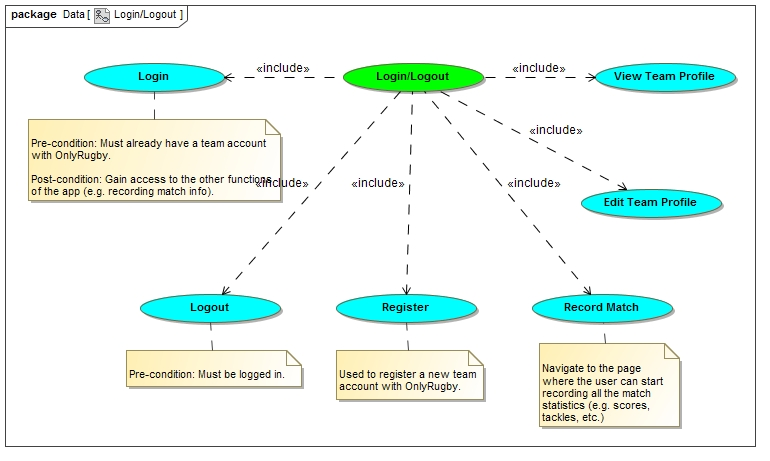
\includegraphics[width=1\textwidth] {./Diagrams/Login_Logout.jpg}\\[0.4cm]    
		\end{center}
\newpage
\item \textbf{Load info}
		\begin{flushleft}
			The Load Info module will be used to transfer information to and from the database, using the server. All destinations are to be verified before attempting to access them and incoming connections to the server need to be verified that they are from a trusted source.
		\end{flushleft}
		\begin{center}
  	 	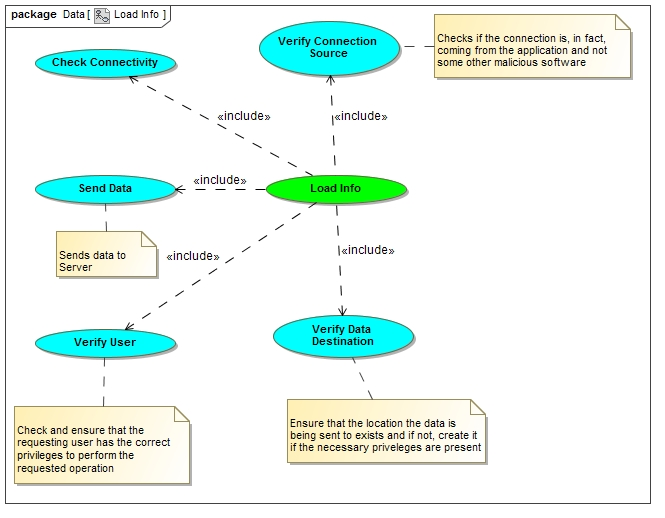
\includegraphics[width=1\textwidth] {./Diagrams/LoadInfo.jpg}\\[0.4cm]    
		\end{center}
\newpage\item  \textbf{Game time}
		\begin{flushleft}
		 This use case will be used to log the start and end time of each half of a match, as well as any intervals during which time was lost (the game was paused) and a reason for this time loss (injury, substitution, referee consultation, replacement of damaged player clothing).	
		\end{flushleft}
		\begin{center}
  	 	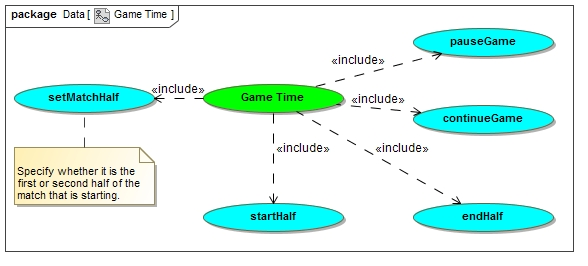
\includegraphics[width=1\textwidth] {./Diagrams/Game Time.jpg}\\[0.4cm]    
		\end{center}
\newpage
\item \textbf{Scoring}
		\begin{flushleft}
		 This use case deals with logging, verifying and storing all the information related to scoring points during a match. When a player scores during a match the app user must use this use case to specify which team scored, the individual player who scored, if the player scored with a try, drop kick, penalty kick or conversion  kick and (in the case of the try) if any other players should be credited with a try assist. This use case will also automatically log when the points were scored. All this information is then verified by the app user before it is stored in the database. Once stored this information can then be used to give team- and player statistics.	
		\end{flushleft}
		\begin{center}
  	 	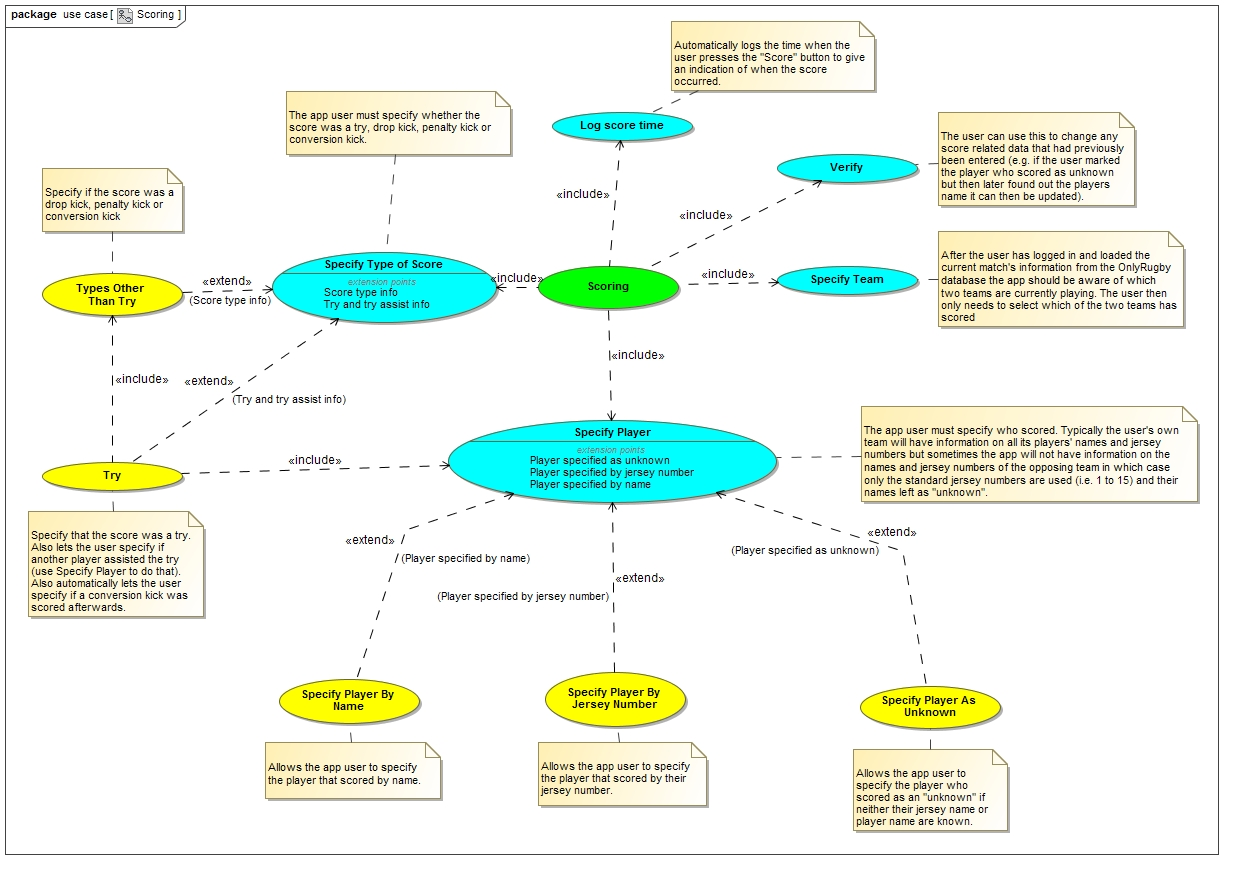
\includegraphics[width=1\textwidth] {./HermanDiagrams/Scoring.jpg}\\[0.4cm]    
		\end{center}
\newpage
	\item \textbf{Substitutions}
		\begin{flushleft}
		 This use case deals with logging and updating any changes made to either teams on-field teams. When a team makes a substitution the user of the OnlyRugby app will use this use case to specify which team made the substitution, which players were swapped and if there was any special reason for the substitution. This use case will also automatically log when a player has been swapped. All this information is then verified by the app user before it is stored in the database. Once stored this information can then be used to give team- and player statistics.
		\end{flushleft}
		\begin{center}
		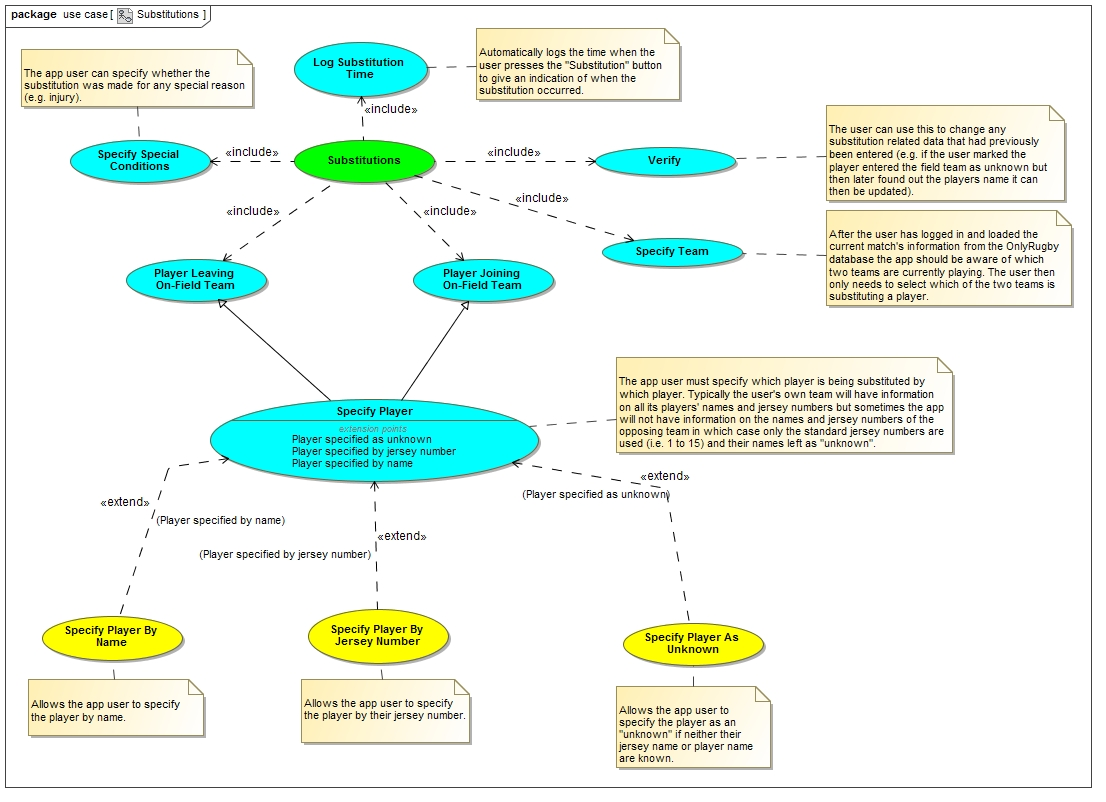
\includegraphics[width=1\textwidth]{./HermanDiagrams/Substitutions.jpg}\\[0.4cm]
		\end{center}
\newpage
	\item \textbf{Discipline}
		\begin{flushleft}
		This use case will be used to log any infractions and subsequent punishment for players. If a player is given a card, the reason for the card, as well as the colour of said card. This data will then be logged to the player's profile.
		\end{flushleft}
		\begin{center}
		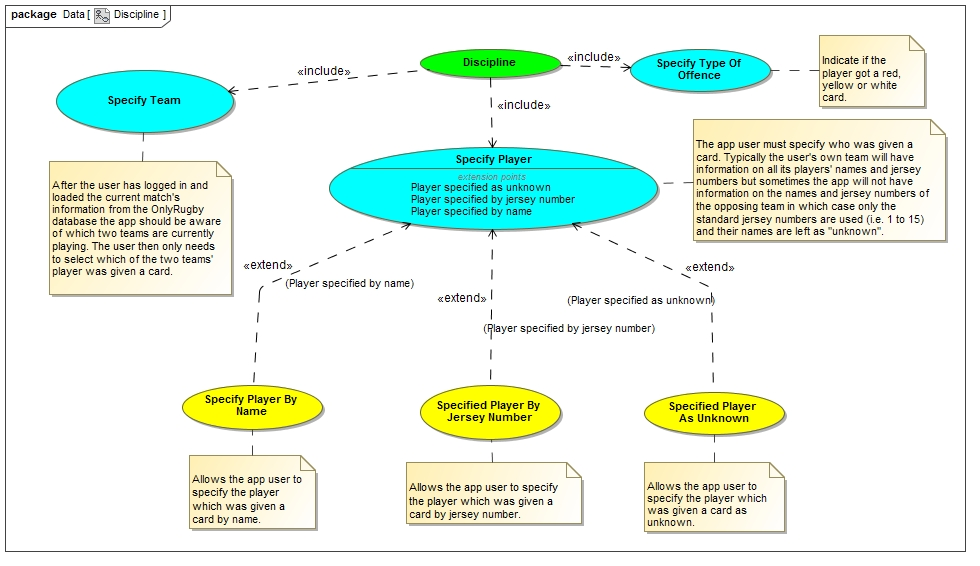
\includegraphics[width=1\textwidth]{./Diagrams/Discipline.jpg}\\[0.4cm]
		\end{center}
\newpage
	\item \textbf{Lineouts}
		\begin{flushleft}
		This use case will be used to log information on when a lineout occurred, which team was responsible for throwing in the ball, the identity (name or player number) of the player that threw in the ball, whether or not the lineout was successful, if successful which team won the lineout, and if unsuccessful a reason why the lineout failed.
		\end{flushleft}
		\begin{center}
		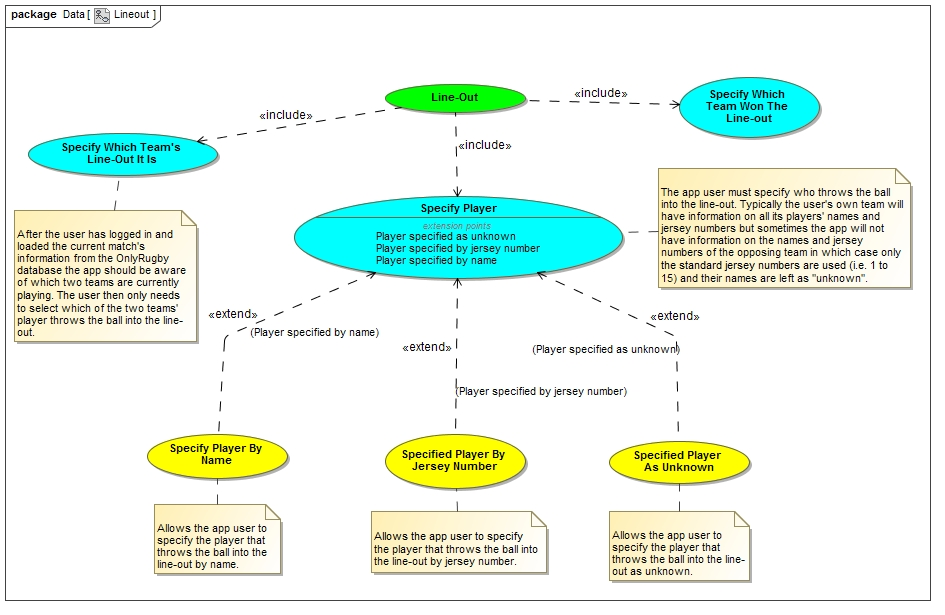
\includegraphics[width=1\textwidth]{./Diagrams/Lineout.jpg}\\[0.4cm]
		\end{center}
\newpage
	\item \textbf{Scrums}
		\begin{flushleft}
		This use case will be used to log information on when a scrum occurred, which team the scrum belonged to and which team won the scrum. The app can check if there are any current reserves on for any forwards or scrum half, and with this info record who was in the scrum.
		\end{flushleft}
		\begin{center}
		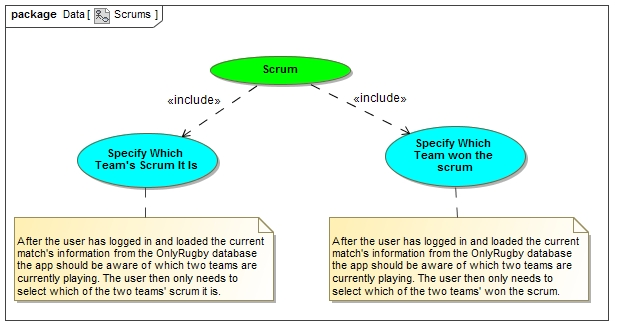
\includegraphics[width=1\textwidth]{./Diagrams/Scrums.jpg}\\[0.4cm]
		\end{center}
	\item \textbf{Tackles}
		\begin{flushleft}
			This use case will be used to log the amount of tackles made, by which team member of which team and when it was made. Knowing who was tackled is not required, since it will not be recorded in their statistics.
		\end{flushleft}
		\begin{center}
		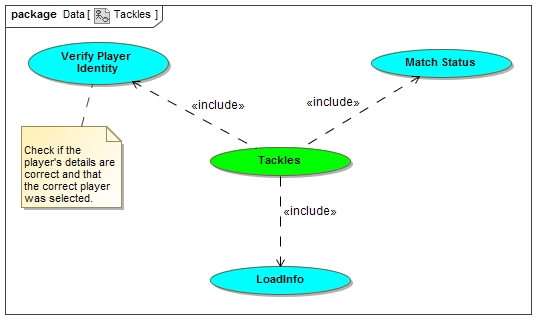
\includegraphics[width=0.9\textwidth]{./Diagrams/Tackles.jpg}\\[0.4cm]
		\end{center}
	\item \textbf{Possession}
		\begin{flushleft}
		This use case will be used to log the percentage of each team's possession for a match. The application will ensure that the total percentages cannot exeed 100 percent.
		\end{flushleft}
		\begin{center}
		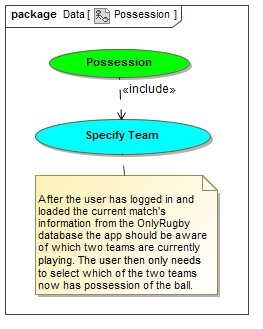
\includegraphics[width=0.4\textwidth]{./Diagrams/Possession.jpg}\\[0.4cm]
		\end{center}
	\item \textbf{Turn-overs}
		\begin{flushleft}
		This use case will be used to log the occurrence of a turn-over, which team got the ball, which team lost the ball and the players who were involved in the turn-over.
		\end{flushleft}
		\begin{center}
		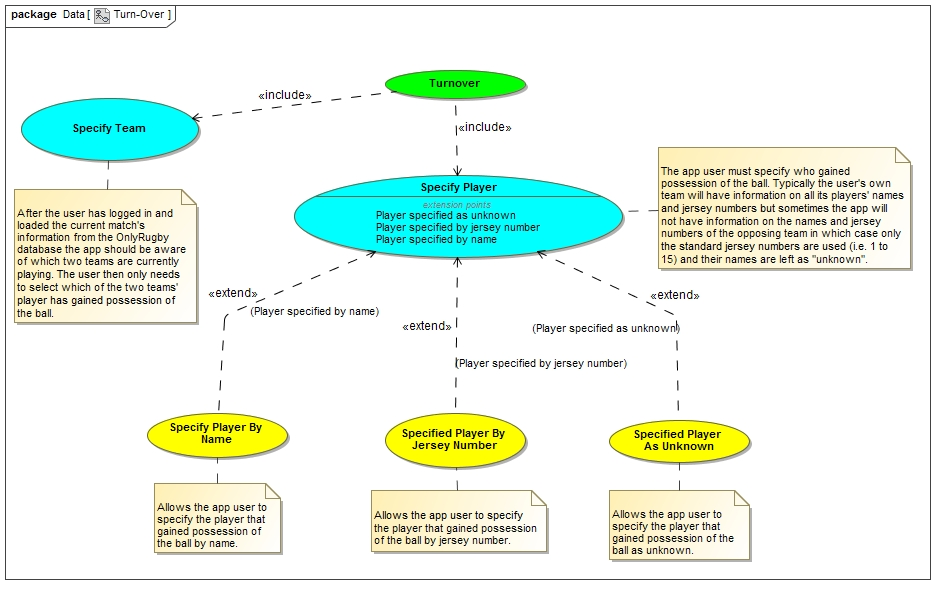
\includegraphics[width=1\textwidth]{./Diagrams/Turn-Over.jpg}\\[0.4cm]
		\end{center}
	\item \textbf{Clean breaks}
		\begin{flushleft}
		This use case will be used to log when clean breaks occur, the player that got the clean break will also be recorded.
		\end{flushleft}
		\begin{center}
		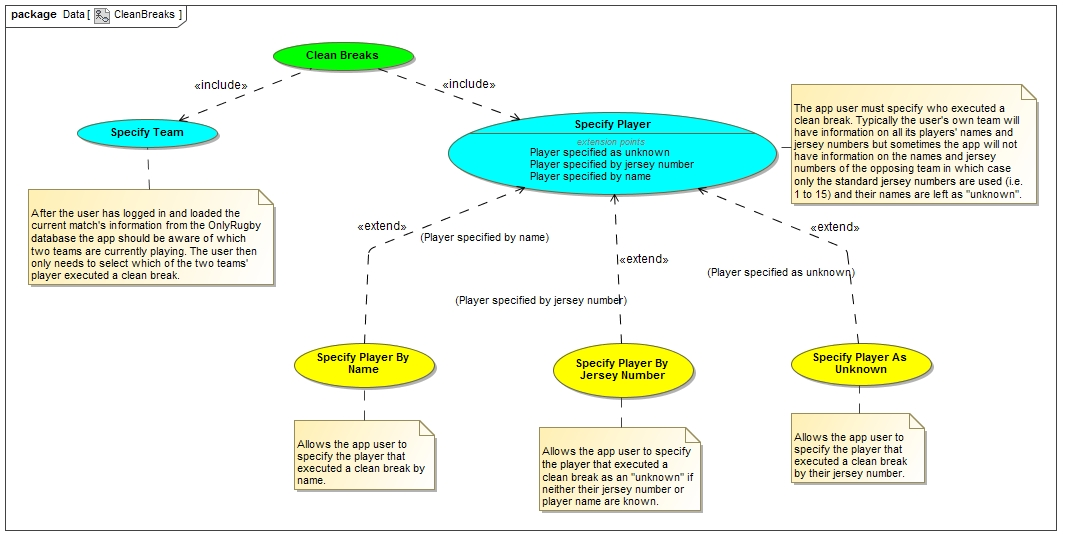
\includegraphics[width=1\textwidth]{./Diagrams/CleanBreaks.jpg}\\[0.4cm]
		\end{center}
	\item \textbf{Offloads}
		\begin{flushleft}
		This use case will be used to log information on when an offload occurs, which team performed the offload, and the identity (name or player number) of the player that performed the offload.
		\end{flushleft}
		\begin{center}
		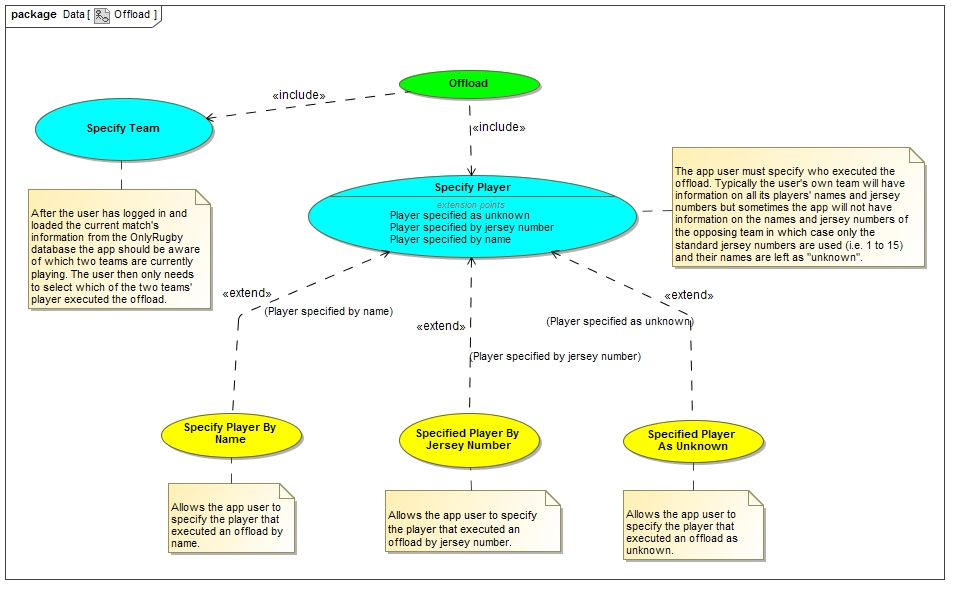
\includegraphics[width=1\textwidth]{./Diagrams/Offload.jpg}\\[0.4cm]
		\end{center}
	\item \textbf{Rucks}
		\begin{flushleft}
		This use case deals with logging any instance of a ruck during match time. When a ruck occurs during a match the OnlyRugby app user can then use this use case to specify which team was defending during the ruck and whether possession of the ball changed during/after the ruck. This use case will also automatically log when a ruck occurs. All this information is then verified by the app user before it is stored in the database. Once stored this information can then be used to give team- and player statistics.
		\end{flushleft}
		\begin{center}
		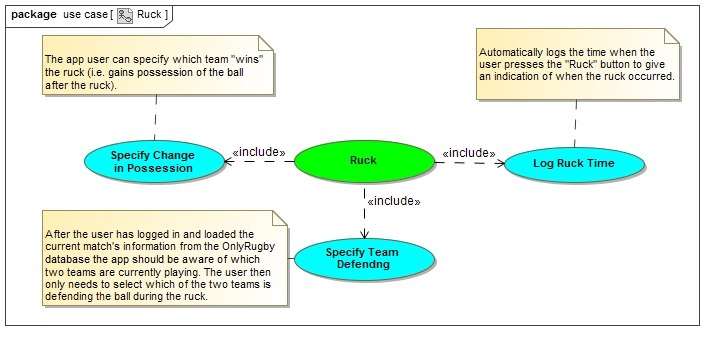
\includegraphics[width=1\textwidth]{./HermanDiagrams/Ruck.jpg}\\[0.4cm]
		\end{center}
\newpage
	\item \textbf{Mauls}
		\begin{flushleft}
			This use case will be used to log how many mauls occurred throughout the match. It will record how many occurred, when they occurred and who won the outcome of the maul (whether there was a turnover ball or not, or if a penalty was conceded).
		\end{flushleft}
		\begin{center}
		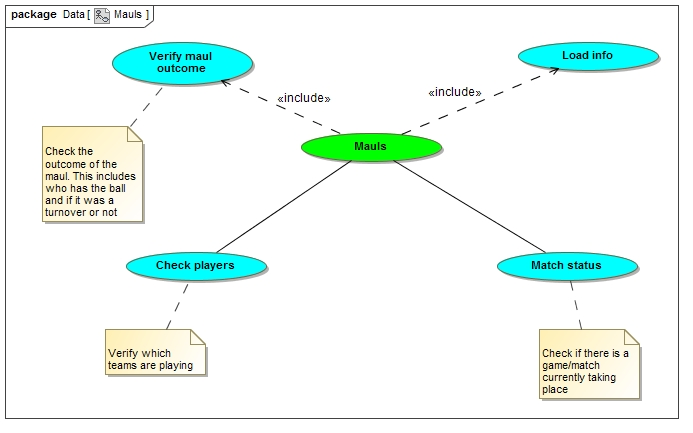
\includegraphics[width=1\textwidth]{./Diagrams/Mauls.jpg}\\[0.4cm]
		\end{center}

	\item \textbf{Events List}
		\begin{flushleft}
			This use case will allow the user to view a time-sorted list of events that have so far been logged in the match. It will also facilitate the alteration and deletion of these events as well as the addition of new events to the list. Once an event has been deleted or altered all the previously logged information of that event will be erased (and in the case of alteration, be replaced with new log info).
		\end{flushleft}
		\begin{center}
		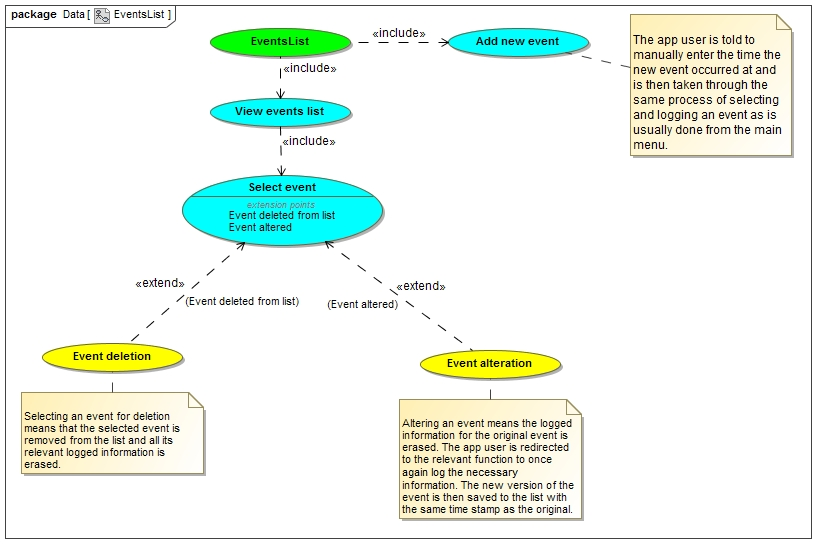
\includegraphics[width=1\textwidth]{./Diagrams/EventsList.jpg}\\[0.4cm]
		\end{center}
\end{itemize}
\newpage
\subsection{Process specification}
The processes followed when using some of the more important functions of the OnlyRugby app system are displayed below:
\begin{itemize}
	\item Log in/ log out
		\begin{center}
  	 	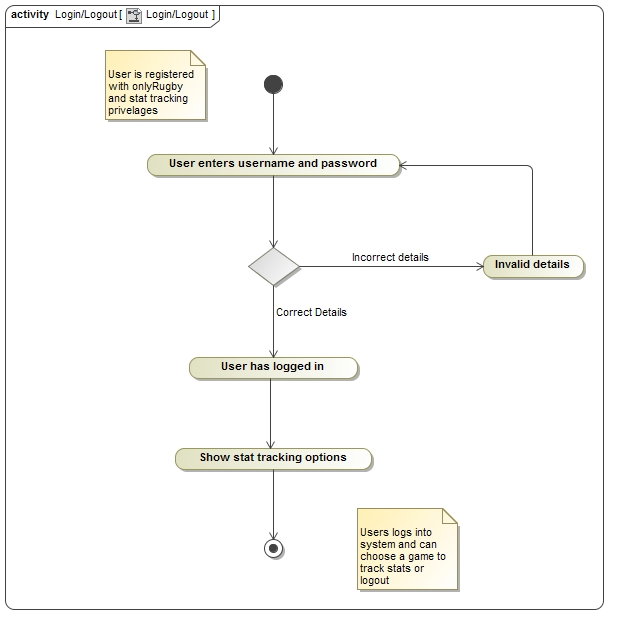
\includegraphics[width=0.6\textwidth] {./Diagrams/Login_LogoutActivityDiagram.jpg}\\[0.4cm]    
		\end{center}
	\item Load info
		\begin{center}
  	 	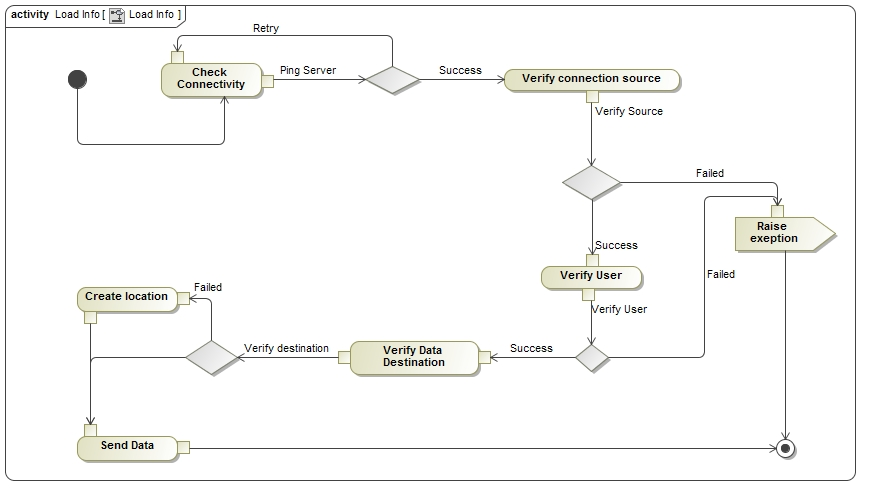
\includegraphics[width=1\textwidth] {./Diagrams/LoadInfoActivityDiagram.jpg}\\[0.4cm]    
		\end{center}
	\item Game time
		\begin{center}
		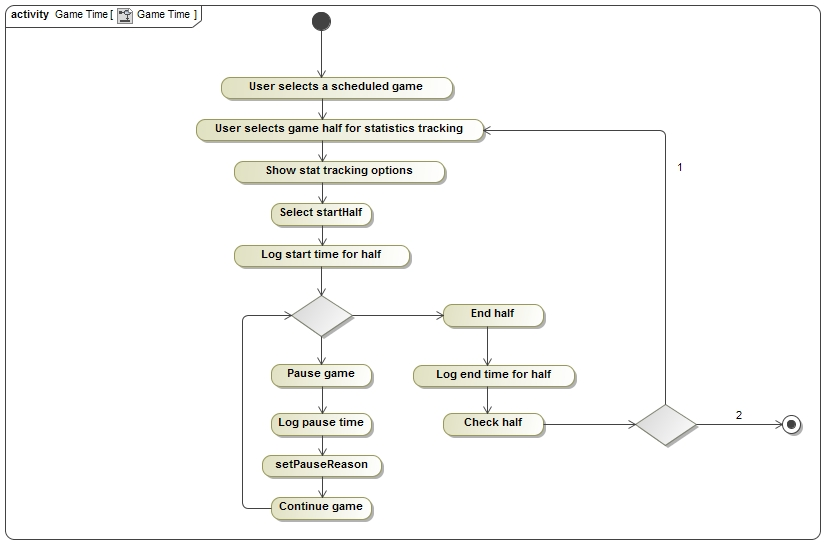
\includegraphics[width=1\textwidth] {./Diagrams/GameTimeActivityDiagram.jpg}\\[0.4cm]
		\end{center}
	\item Scoring
		\begin{center}
		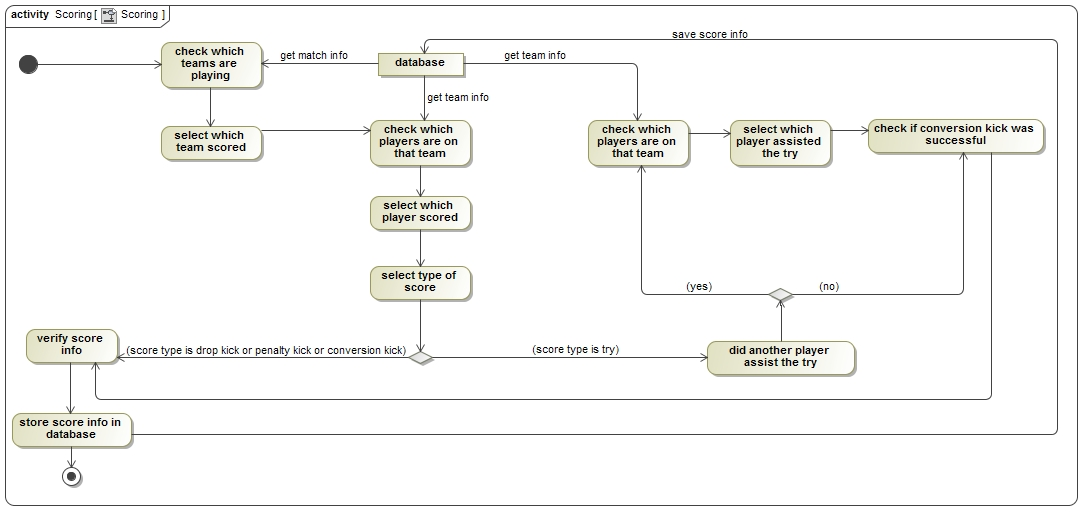
\includegraphics[width=1\textwidth] {./HermanDiagrams/ScoringActivityDiagram.jpg}\\[0.4cm]
		\end{center}
\newpage
	\item Substitutions
		\begin{center}
		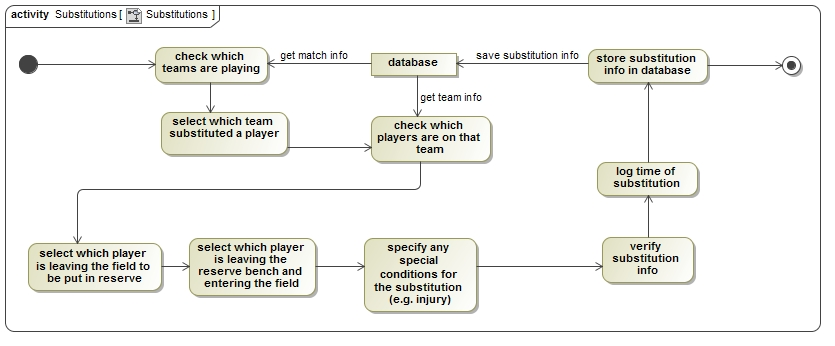
\includegraphics[width=1\textwidth] {./HermanDiagrams/SubstitutionsActivityDiagram.jpg}\\[0.4cm]
		\end{center}
	\item Discipline
		\begin{center}
		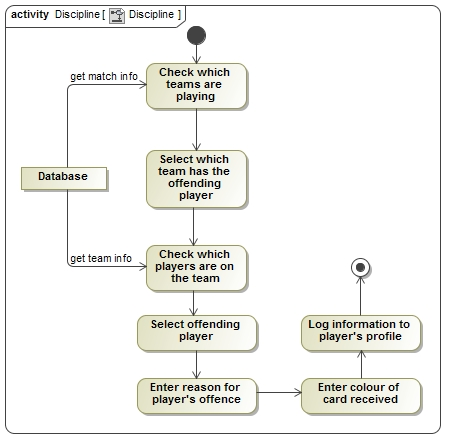
\includegraphics[width=0.6\textwidth] {./Diagrams/DisciplineActivityDiagram.jpg}\\[0.4cm]
		\end{center}
\end{itemize}
\subsection{Domain Model}
	\begin{center}
  	 	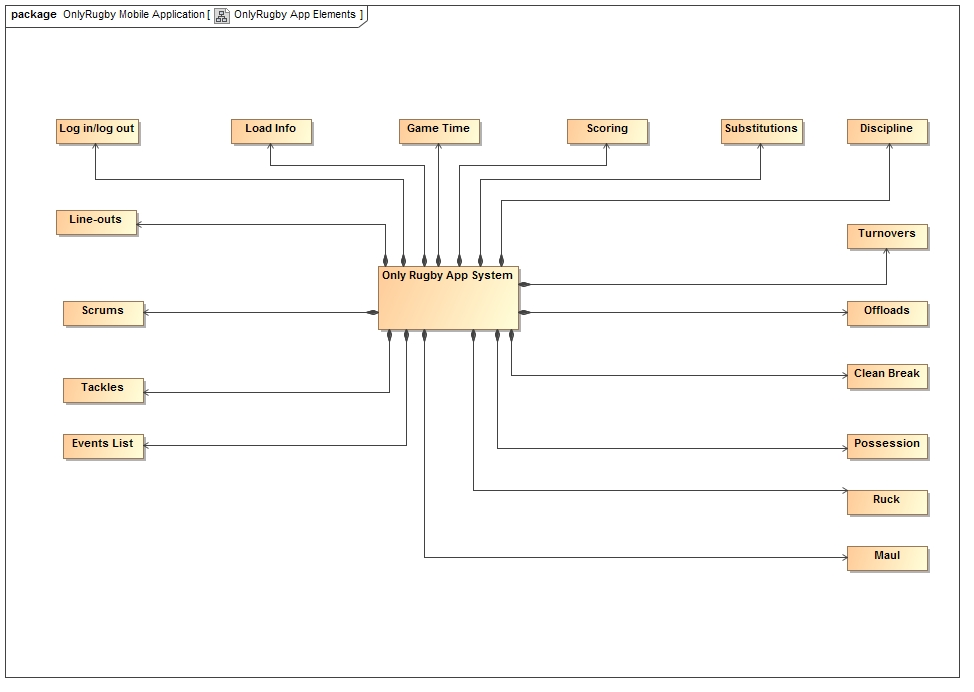
\includegraphics[width=1\textwidth] {./HermanDiagrams/DomainModel.jpg}\\[0.4cm]    
	\end{center}
\index{Vision}

\end{document}
